\chapter{Optimization}

The solution presented in Chapter~\ref{chap:solution}, despite
providing correctness guarantees and ease of use, performs poorly in
even trivial test cases. This chapter describes a series of
optimizations made to keep the overhead as low as possible, without
sacrificing correctness.

\section{Example Application}

To perform accurate measurements, a sample banking application was
developed. In this application's domain there is a central Bank with
Customers, which in turn have their accounts. For each account there
is a slot representing the account's balance, and there is a method to
show a customer's balance (by summing the balance of all his
accounts). Every time a transaction is done, a new TransactionRecord
is created, containing a timestamp, the origin and destination
accounts, as well as the amount transfered.

In this scenario, a Business Transaction will be made of several
banking transactions throughout a series of steps. This is the perfect
candidate for a Long Lived Transaction.

With the support presented in previous sections, the programmer simply
writes the application's code as he would without considering Long
Lived Transactions. No changes to the data structures and business
logic are required.

Using this banking domain, a sample application was developed. In this
fictitious scenario, the bank would start with a certain number of
customers (this number was configurable so different parameters could
be measured), create a Long Lived Transaction with a configurable
number of steps. Within each step, new customers and accounts would be
created, money would be shuffled between all the bank's accounts
(creating a new TransactionRecord for each transaction), and the total
balance is calculated. This means that in each step: 1) Every object
is read, 2) Many objects are written, 3) Many objects are created.

\section{Initial Performance Analysis}

Figure~\ref{fig:regTime} shows the running time for a varying number
of iterations on the application presented above. As expected, the
running time grows linearly as the number of iterations increases.

When looking at the Long Lived version (where every iteration is a
step of a large Long Lived Transaction), performance quickly degrades
as the number of iterations grows {\it O(n3)}. The main reason for
this performance hit is that every read box will cause many other
boxes to be read (instead of just reading the box directly, the whole
write set must be traversed, meaning that many more boxes are read
along the way, and many more boxes will be read as the transaction
grows in size). Recall from Chapter~\ref{chap:ff} that in the JVSTM
using a multi-box layout, each slot of an object is kept in a separate
box, and as such reading a single Log Entry will cause at least 3
boxes to be read: the slot name, the target object, and the next box
in the list.

Figure~\ref{fig:reg-box} shows that in a regular transaction, the
number of read boxes is linear to the number of iterations, matching
the linear running time. The same behaviour is observed with Long
Lived Transactions. Figure~\ref{fig:long-box-v1} shows that the number
of boxes read grows following the same pattern as the running time.

As reading boxes is one of the major sources of the poor performance
results of the implementation, various improvements were made to both
improve reading boxes and reduce the number of boxes read. The next
sections present those optimizations.

\begin{figure}
\centering
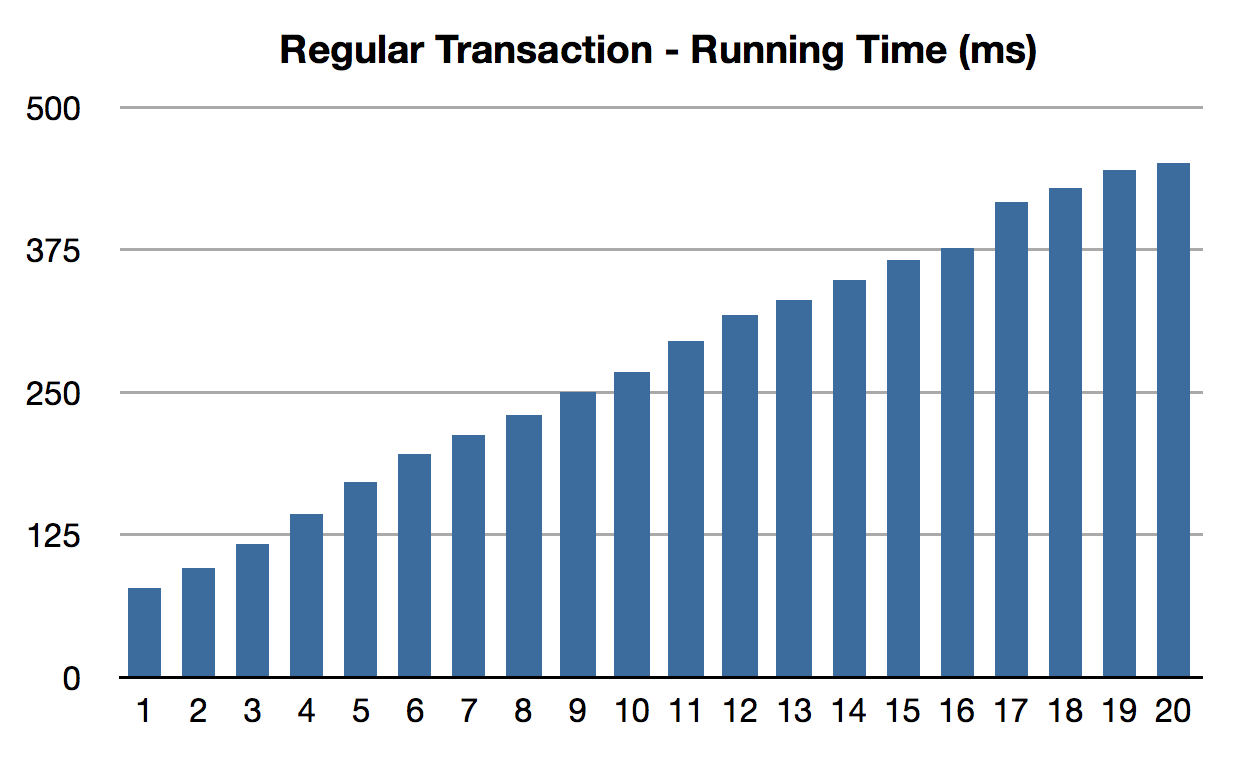
\includegraphics[width=0.7\linewidth]{reg-time}
\caption{Running time with regular transactions}
\label{fig:regTime}
\end{figure}

\begin{figure}
\centering
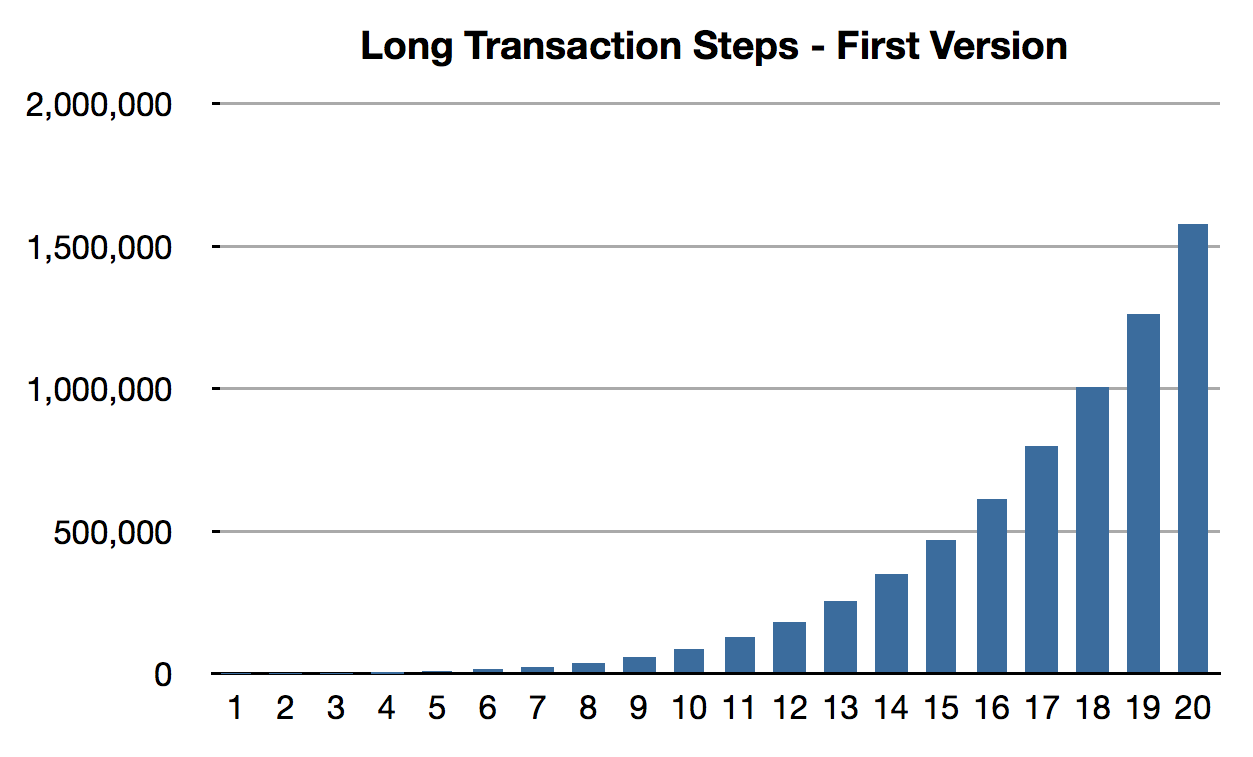
\includegraphics[width=0.7\linewidth]{long-time-v1}
\caption{Running time with Long Lived Transaction steps}
\end{figure}

\begin{figure}
\centering
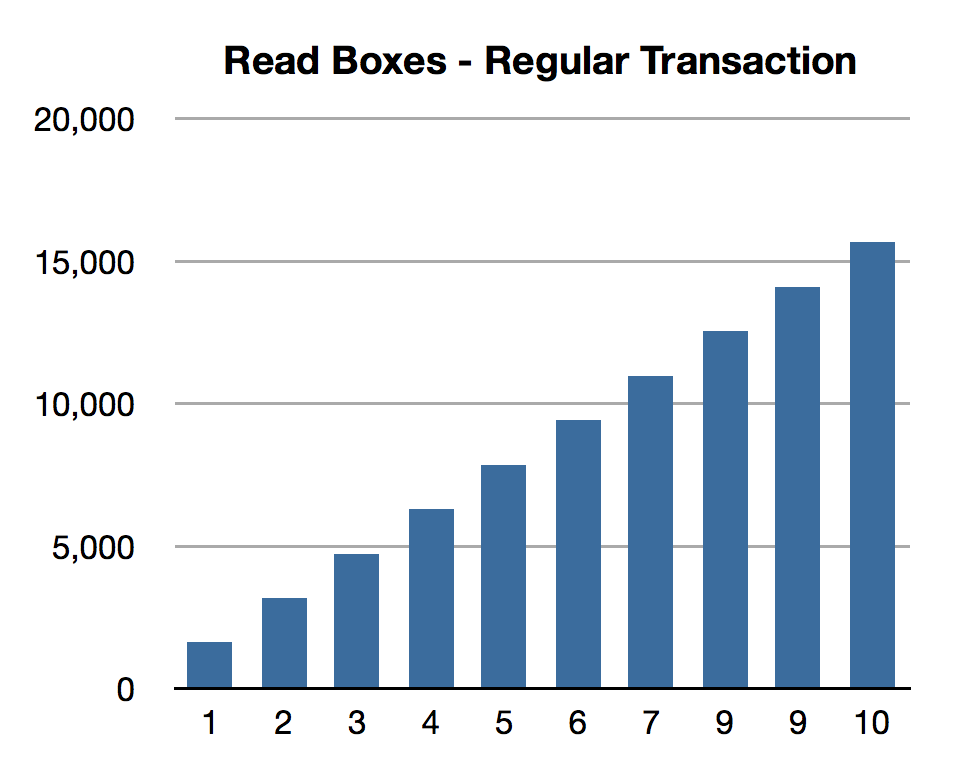
\includegraphics[width=0.6\linewidth]{reg-box}
\caption{Number of boxes read on a regular transaction}
\label{fig:reg-box}
\end{figure}

\begin{figure}
\centering
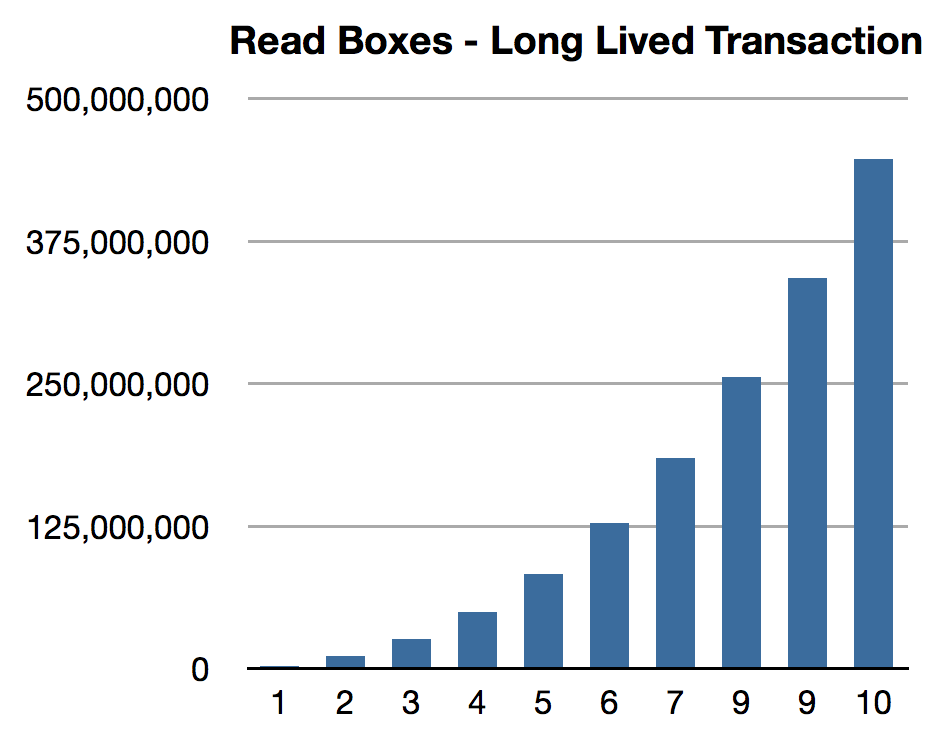
\includegraphics[width=0.6\linewidth]{long-box-v1}
\caption{Running time with Long Lived Transaction steps}
\label{fig:long-box-v1}
\end{figure}

\section{Read-Set differentiation}

In the initial implementation, {\it LogEntries} were used to reify
both the Read Set and the Write Set.

Recalling Figure \ref{fig:architecture}, {\it LogEntries} store a
reference to the DomainObject they refer to, the name of the slot, and
the slot's value. Using the same objects to represent both sets proved
to be quite expensive, as the Read Set only cares about which slots
were read, completely ignoring its value.

Carefully looking at the nature of the Read Set, one comes to realise
that it is only necessary to store the pairs [DomainObject, Slot] read
by the transaction (the actual version read is not relevant, as it
will always be coherent with the transaction's version).

As such, the Read Set has been replaced by an immutable
ValueType\footnote{ValueTypes are explained in detail in Chapter
  \ref{chap:ff}}, containing a set of DomainSlotKey's (an immutable,
lightweight object representing the pair [DomainObject, Slot]), stored
directly into the {\it TransactionalContext}.

This optimization greatly reduced the space required by the
Transaction (both in-memory and persistently), as the representation
of the Read-Set became more compact (a single slot in an object vs
several objects).

The commit time for the various steps of the Transaction also
improved, as the lookups/insertions of entries in the Read Set are
done entirely in memory, without the need to traverse (and
potentially reload a large object graph).

\section{Using BPlusTrees to hold LogEntries}

As described in Chapter \ref{chap:ff}, the Fenix Framework uses
BPlusTrees and other collections to implement to-many relations. These
collections are transparently handled by the Framework, and are
implemented using regular Domain Objects (such as Leaf Nodes and Inner
Nodes). It is then desirable to store the correct values of those
objects within the context of a Long Transaction, as changes in
relations are part of our transparent programming model.

This posed a great issue, as conceptually one {\it
  TransactionalContext} has many {\it LogEntries} in both its Read and
Write Sets. If this relation ware to be implemented using a regular
one-to-many relation, a BPlusTree would be generated by the
Framework. But as BPlusTrees cannot be kept out of the
TransactionalContext, they could not be used to implement this relation.

The initial solution consisted on implementing the relation using a
Linked List, in which a LogEntry would be directly connected to the
next one in the list, keeping the list sorted by insertion
order. Figure~\ref{fig:linkedList} shows how this was designed..This
approach proved to be quite inefficient, as lookups in the Write Set
were {\it O(n)} in the number of written objects, making it
impractical, as every {\it getBoxValue} operation required potentially
traversing the whole list.

\begin{figure}
  \centering
  \begin{tikzpicture}

\begin{class}[text width=5cm]{TransactionalContext}{5,0}
\end{class}

\begin{class}[text width=2cm]{LogEntry}{5,-2}
\end{class}

\begin{class}[text width=2cm]{LogEntry }{10,-2}
\end{class}

\association{TransactionalContext}{}{}{LogEntry}{writeSet}{0..1}
\unidirectionalAssociation{LogEntry}{nextEntry}{}{LogEntry }

\end{tikzpicture}

\caption{}
\label{fig:linkedList}
\end{figure}

To solve this issue, a specialised WriteSetBPlusTree was
developed. The major difference a WriteSetBPlusTree and a regular
BPlusTree is that the former is designed to be kept out of the scope
of the TransactionalContext, making it possible to use to implement
the one-to-many relation between a TransactionalContext and its
LogEntries.

Another advantage of directly using a BPlusTree is that it is possible
to take full advantage of all its features. Generically speaking, a
BPlusTree is a map between keys and values. When the Fenix Framework
generates a BPlusTree to represent a to-many relation, the map
contains the pointed objects as values, and the object's identifiers
(OID) as keys. In this case however, lookups are not performed by OID,
but by DomainSlotKey (DomainObject+slot). As such, a WriteSetBPlusTree
will map DomainSlotKeys to their corresponding LogEntries.

With this approach, looking up a DomainSlotKey in a
TransactionalContext means that the BPlusTree is indexed using the
DomainSlotKey, and as such, lookup times are now {\it O(log(n))}.

FIGURAS

\section{Removing LogEntries}

With the relation between the {\it TransactionalContext} and the {\it
  LogEntries} implemented using a BPlusTree, another issue arisen. 

Despite having great lookup times, the commit of a Long Transactions's
step was greatly affected. Whereas inserting elements in a Linked List
is {\it O(1)}, the insertion in the BPlusTree was still painfully
slow.

This is because the Fenix Framework requires that ValueTypes (such as
the ones used to back the BPlusTree) are immutable combined with the
fact that the BPlusTree provides no API for batch insertion, meaning
that for each of the elements written within a given step, a new
insert was performed, and the backing TreeMaps were duplicated over
and over. 

The approach to solve this issue, was to use a solution similar to the
one used for the Read-Set: create an immutable ValueType, containing
the mapping between all written slots and their respective values.

With this change, {\it LogEntries} were completely taken out of the
picture, as the only extra piece of information they provided was the
JSON contents of the slot, which could be embedded directly into the
WriteSet object.

The issue with this approach, is that due to the immutability
requirement, every time a batch of entries was inserted, the whole Map
had to be duplicated, which was rather wasteful both in terms of time
and allocated memory. So, instead of duplicating the whole Map, the
WriteSet is actually a Linked-List of Maps, containing one node per
transaction step. This meant that the performance of lookups is now
{\it O(s*log(n))}, {\it n} being the average size of each step, and
{\it s} the number of steps (in which something is written) of the
transaction.

There is however a tradeoff. Transactions with a small number of large
steps (which is the typical use case) are greatly improved (as lookups
in an in-memory hash map are fast), however transactions with a large
number of small steps take a major performance hit, as a new node is
created in every step with small amounts of information.

As such, a new node is only created if the current node has size above
a certain (user-defined) threshold. This threshold defines whether it
is more cost-effective to create a new node (which is practically
instant on insertion but makes lookups more expensive) or replace the
current one (thus duplicating the map). The user can set the threshold
to be lower or higher according to the usage patterns of the
application.

Applications with a large number of small steps benefit from a large
threshold, as insertions with be quite cheap and have little to no
impact on lookups. On the other hand, applications with a small number
of large steps should set the threshold lower than the average size of
a step, so that it there is no need to duplicate a potentially large
map. 

\section{Final Performance Analysis}

After applying all of the optimizations described in this chapter, the
final solution presents a very competitive performance, keeping the
slowdown factor below 2.
